\documentclass[a4paper, oneside]{memoir}% Document class
\usepackage[a4paper]{geometry}			% Margins
\usepackage{lmodern}
\usepackage{graphicx}
\usepackage{float}
\usepackage{listings}
\usepackage[small,compact]{titlesec}	% No 'chapter' in chapter headings.
\graphicspath{{Media/}}					% Directory that holds images.

\titleformat{\chapter}[hang]
{\normalfont\Large\bfseries}{\thechapter}{1em}{\Large}
\titlespacing{\chapter}{0pt}{*0}{*1}

\titleformat{\chapter}{\Huge\bfseries}{\thechapter}{1em}{}
\titleformat{\section}{\LARGE\bfseries}{\thesection}{1em}{}
\titleformat{\subsection}{\Large\bfseries}{\thesubsection}{1em}{}
\titleformat{\subsubsection}{\normalsize\bfseries}{\thesubsubsection}{1em}{}


\author{
  Erik Sidelmann Jensen\\
  \texttt{ejens11@student.aau.dk}
  \and
  Lasse Vang Gravesen\\
  \texttt{lgrave11@student.aau.dk}
  \and
  Dennis Jakobsen\\
  \texttt{djakob11@student.aau.dk}  
}

\title{Data Intensive Systems - Miniproject - Part 2}
\date{}

\begin{document}
	\clearpage\maketitle
	\thispagestyle{empty}
	
	\chapter{DIS Miniproject}
	\section{Task D}
    We choose to load the data from the provided CSV files, according to the following high-level ETL Flow:
    \begin{figure}[H]
    \begin{center}
    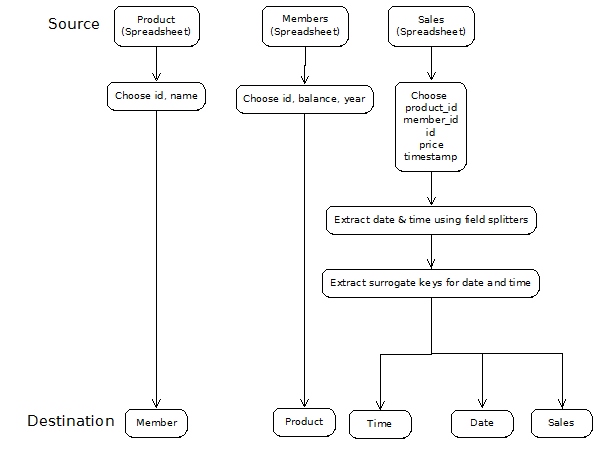
\includegraphics[scale=0.75]{highlevel}
    \caption{High Level ETL Flow}
    \label{fig:HighLevelETLFlow}
    \end{center}
    \end{figure}  
    
    This is the flow it follows in Pentaho (aka Spoon):
    
    \begin{figure}[H]
    \begin{center}
    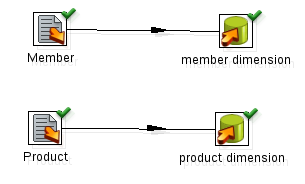
\includegraphics{etlflowmemberproduct}
    \caption{Pentaho ETL Flow for Member and Product}
    \label{fig:PentahoETLFlowMemberAndProduct}
    \end{center}
    \end{figure}
    
    \begin{figure}[H]
    \begin{center}
    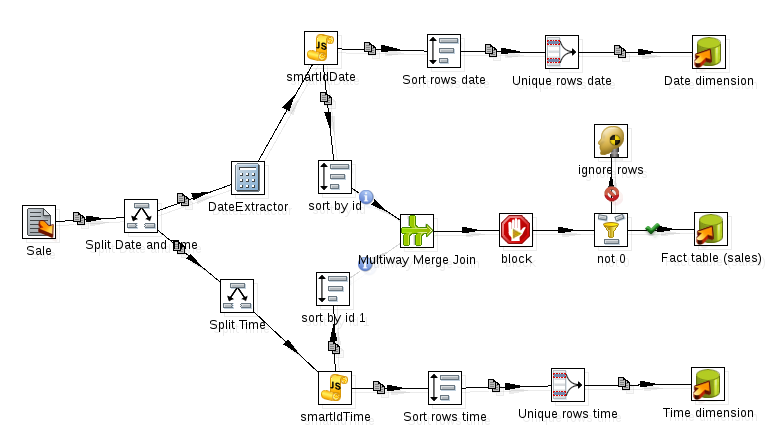
\includegraphics[scale=0.75]{etlflowsales}
    \caption{Pentaho ETL Flow for Sales}
    \label{fig:PentahoETLFlowSales}
    \end{center}
    \end{figure}
       
    The ETL Flow for `sales', `date' and `time' is most interesting, so we go into more detail there. The first step we take is split the timestamp into date and time, by splitting on space. For the date dimension we extract the date from that, and create an easily determinable id such that we do not have to do any lookups. Then we sort the date result on the smart id, and make it unique and add it to the date dimension. Then for the time we also create an easily determinable id, sort it on the smart id and make it unique and put it into the time dimension.
    
    For the sales fact table we reuse the smart ids made for the `date' dimension and `time' dimension, sort on the key 'id' and multiway merge join. Then we block execution of this until the rest of the dimensions have been filled because it needs to refer to foreign keys that not necessarily have been inserted yet. Then we filter out some rows from the `sales' fact table because it has foreign keys that do not match the `member' dimension, send the bad ones to a dummy block and the good ones to the `sales' fact table.
    
    \section{Cut Corners}
    We TRUNCATE CASCADE all tables before running the ETL flow and load all the data fully.
    
    We cut a corner by filtering out rows in the `sales' fact table if it contained a member\_id that equalled 0 by using a simple equation.
    
    It is important to note here that we do not use surrogate keys for the `member', `product' and `sales', as such the result does not support versioning. We did this because we felt that it was not all that important to support versioning for this data warehouse because it's a prototype and because we did not figure out until pretty late that for real data warehouses using those surrogate keys is very important and at that point it would have required large changes to what we had already made.
\end{document}
